\documentclass{beamer}

\mode<presentation>
{
  \usetheme{default}      
  \usecolortheme{default}
  \usefonttheme{default}
  \setbeamertemplate{navigation symbols}{}
  \setbeamertemplate{caption}[numbered]
} 

\usepackage[english]{babel}
\usepackage[utf8]{inputenc}
\usepackage[T1]{fontenc}
\usepackage{lmodern}
\usepackage{graphicx}       % include graphics

\graphicspath{ {images/} }

%definice matematických prostředí
\newtheorem{veta}{Věta}
\newtheorem{lema}[veta]{Lemma}

\title[Deep Snake]{Deep reinforcement learning for Snake}
\author{Louis Martin \& Pierre Stock}
\institute{Ecole Normale Supérieure de Cachan, MVA}


\begin{document}

\begin{frame}
  \titlepage
\end{frame}


\begin{frame}{Summary}
  \tableofcontents
\end{frame}

\section{Introduction}

\subsection{Historical reinforcement learning on games}
\begin{frame}{Introduction}{TD-Gammon}
% One of the first successful end-to-end reinforcement reinforcement learning algorithm applied games was TD-Gammon \cite{tesauro1995temporal}.
% The algorithm achieved Super-human performance more than 20 years ago.
  \begin{center}
    \Large Reinforcement learning on games:\\ TD-Gammon in 1992
  \end{center}
    \begin{figure}[!htbp]
    \centering
      \includegraphics[width=0.4\linewidth]{td_gammon.png}
      \caption{TD-Gammon algorithm from \cite{tesauro1995temporal}}
    \end{figure}
\end{frame}

\subsection{working with images}
\begin{frame}{Introduction}{Working with images}
  % Working with high dimensional data such as raw images proves to be a very difficult problem that was usually handled by designing tailor-made low dimensional features that would represent the environment as accurately as possible.
  \begin{itemize}
    \item Images as input: Hard problem, high dimensional states.
    \item Historically: Hand crafted low dimensional features
    \item Recent revival of convolutional networks
  \end{itemize}

  \begin{figure}[h]
  \centering
    \includegraphics[width=\linewidth]{atari.png}
    \caption{Screen shots from five Atari 2600 Games: (Left-to-right) Pong, Breakout, Space Invaders,
  Seaquest, Beam Rider, taken from \cite{mnih2013playing}}
  \end{figure}
\end{frame}

\begin{frame}{Introduction}{Policy gradients}
  \begin{center}
    \Large Policy gradients gained interest over Deep Q-learning.
  \end{center}
  \begin{figure}[!htpb]
    \centering
    \includegraphics[width=.5\linewidth]{alphago.jpg}
    \caption{AlphaGo against the world champion of the game of Go \cite{silver2016go}}
    \label{network}
  \end{figure}
\end{frame}


\section{Theory}

\subsection{Notations and Background}

\begin{frame}{Notations and Background}


%Our agent is the snake from the well-known eponymous game. It interacts with the environment $\mathcal E$ to gets its current state $s_t$ which is a $N \times N$ grid. The initial state at the beginning of one game $s_0$ is the following: the snake has a length of 3 pixels and starts from the left-upper corner of the grid, its head being the rightmost part of its body and a fruit appears randomly in one pixel of the grid where the snake is not (see Fig \ref{snake_init}). Note that the fruit does not disappear until the snake has eaten it. The goal of the game is to eat as many fruits as possible in one game. 
\begin{itemize}
\item Current state $s_t = N \times N$ grid, action state $\mathcal A =$ \{up, down, left, right\}. 

\item Each action $a_t$ modifies the state and triggers a reward $r_t$ : \{{eat}: $-10$, {hit}: $-10$, {fruit}: $+10$, {nothing}: $-1$\} 

\item Goal of the agent: find optimal policy $\pi^{\star}$ that maximizes \[R_t = \sum_{t' = t}^T \gamma^{t' - t} r_{t'}\]

%Using this notion, we can express the goal of the game more formally: the goal of the agent is to \textit{maximize the expected return} from each state $s_t$ by computing the optimal policy $\pi^{\star}$.

%\item $\pi$ maps each state $s_t$ to a probability distribution over the action state $\mathcal A$
\end{itemize}

\begin{figure}[h]
\centering
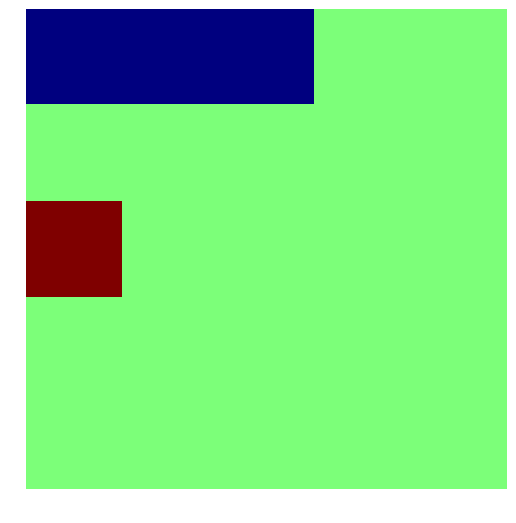
\includegraphics[width=.3\linewidth]{snake_initial_state.png}
\caption{Initial state of the game for $N = 5$}
\label{snake_init}
\end{figure}

\end{frame}

\subsection{Policy Networks}

\begin{frame}{Policy Networks, introduction}

\textbf{Challenges}: detect motion, exploration/exploitation dilemma

%The training goes as follows. After initializing the network, we play a first game by successively feeding the tuple of the last two states $(s_{t-1}, s_t)$ to the policy network (forward pass), sampling action $a_t$ from the output probabilities and updating the new state of the game $s_{t + 1}$ until the game is over.

%Our agent will be implemented by a policy network that will take the state of the game $s_t$ as input and output 4 probabilities corresponding to the policy $\pi_t$. For the network to be able to detect motion (and where the head of the snake is), we actually feed it with the last two frames $(s_{t-1}, s_t)$, where $s_{-1}$ is the grid filed with zeros. 

%We first experimented a fully connected network with 1 hidden layer of size $n_h$, taking as input $2 * N^2$ pixels and outputting $4$ values, stacked with a softmax layer to output probabilities. The structure of this network is illustrated in Fig \ref{network}. In this example, the network will output very low probabilities for going up (eating itself) or going down (hitting the wall), and will be more likely to go to the left than to the right due to the presence of the fruit on the right side, and because going to the left will definitely lead to game over. 

\begin{figure}[!htpb]
\centering
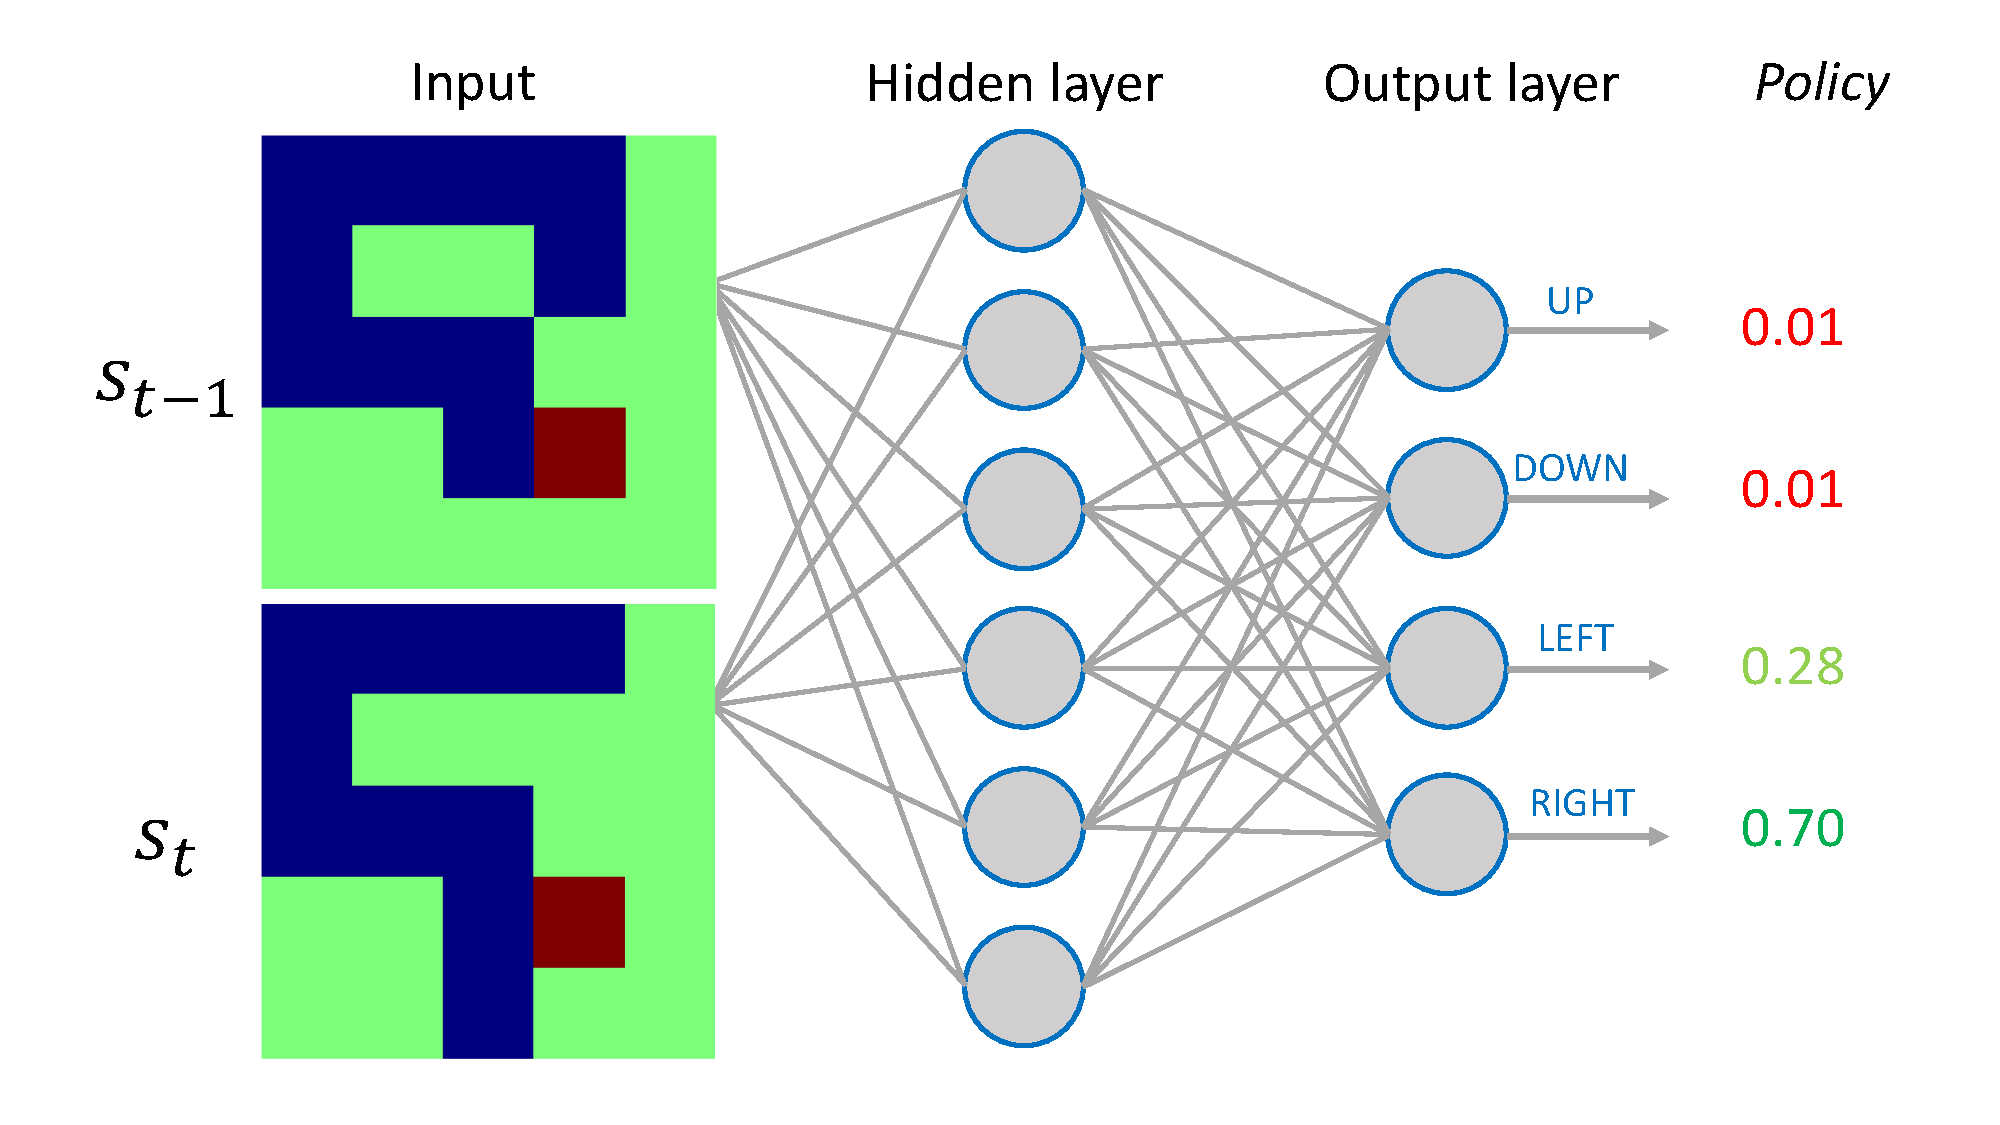
\includegraphics[width=\linewidth]{layer.pdf}
\caption{Network architecture}
\label{network}
\end{figure}

\end{frame} 

\begin{frame}{Policy Networks explained}

\textbf{Idea}: learn the policy by playing batches of games and updating the network parameters by backpropagation afterwards when we know if a particular move was conclusive 
 

\begin{figure}[!htpb]
\centering
\includegraphics[width=\linewidth]{algo.png}
\caption{General Policy Gradient Algorithm}
\label{algo}
\end{figure}

\end{frame}

\begin{frame}{Policy Networks explained}

\begin{itemize}

\item Loss function depending on the batch

%To do that, we have to define a loss function assessing whereas a particular action $a_t$ in a particular game  of the batch was rather \textit{good} or \textit{bad}. Let us note $x_{i, t} = (s_{i, t - 1}, s_{i, t})$ where $s_{i,t}$ is the state of the $i^{th}$ game of the batch at time $t$, $y_{i, t}$ the action that was sampled from the policy network after the forward pass of $x_{i, t}$ and $R_{i, t}$ the expected return at time $t$ of the action $y_{i, t}$, that is, 

%\[R_{t, i} = \sum_{t' = t}^{T_i} \gamma^{t' - t} r_{t'}\]

%where $T_i$ is the length of the $i^{th}$ game. Then, the loss function for that particular batch $k$ writes

\[\ell_k = - \sum_{i = 1}^{n_b} \sum_{t = 1}^{T_i} R_{i, t} \log p(y_{i, t} | x_{i, t})\]
with $p(y_i | x_i)$ is the probability of action $y_i$ given by the network when it sees input $x_i$,  $R_{i, t}$ the expected return at time $t$ of the action $y_{i, t}$.
%where $p(y_i | x_i)$ is the probability of action $y_i$ given by the network when it sees input $x_i$. Note that the loss function \textit{varies} from batch to another to adapt to the games that were played. 

\item $R_{t, i} = $ \textit{advantage} of the game $i$ at time $t$, depends on the discount factor $\gamma$. %Low values of $\gamma$ will lead to \textit{short-sighted} policies whereas high values of lambda will lead to \textit{long-sighted} policies. 

\item Normalize the expected rewards $R_{i, t}$ per batch
\begin{itemize}
\item Diminish the variance of the gradient% when backpropagating and thus ensures a more stable learning process 
\item Roughly half of the games of the batch \textit{bad} the other \textit{good}%. This is of course not the case in practice but this has significantly improved our experimental results. 
\end{itemize}
\end{itemize}

\end{frame}

\section{Experiments}
\subsection{Network architecture \& Setup}

\begin{frame}{Network architecture \& Setup}

\begin{itemize}
\item Python implementation available online\footnote{GitHub repo: \url{http://github.com/RLSnake/Snake}}{}.

\item \textbf{Parameters}: learning rate, set of rewards, batch size, hidden layer size, grid size, $\gamma$, number of  iterations

\item Each set of parameters was run for 10.000 games

\item We experimentally observed low inter-training variability %was small so we ran each set of parameter only once to get good qualitative results.

\item \textbf{Performance measure}: number of time the Snake played without loosing, along with the number of fruits eaten

\item To avoid infinite loops,  we set a constraint on the time spent without eating fruits ($3 \times grid\_size$ actions) after which the game is lost %, it lost the game. This ensures that the snake has to eat fruits in order to keep playing a get a higher reward. %In order to prevent the lifetime measure to be impacted by a algorithm that would loop over to avoid the walls without actually trying to eat the fruit, we set a constraint on the time spent without eating fruits.



\end{itemize}

\end{frame}

\subsection{Results}

\begin{frame}{Demo}
  \begin{center}
  \Huge Show time !
  \end{center}
\end{frame}

\begin{frame}{Results}{Parameter exploration}
\begin{figure}[!htpb]
\centering
  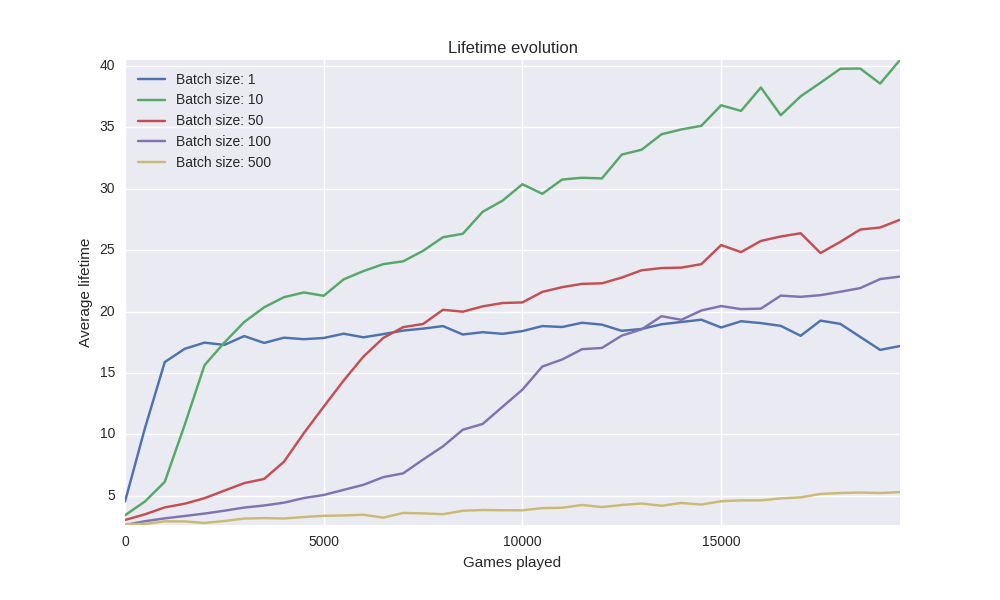
\includegraphics[width=\linewidth]{batch_size_dependence.png}
  \caption{Influence of the batch size}
  \label{batch_size}
\end{figure}
\end{frame} 

\begin{frame}{Results}{Parameter exploration}
\begin{figure}[b]
\centering
  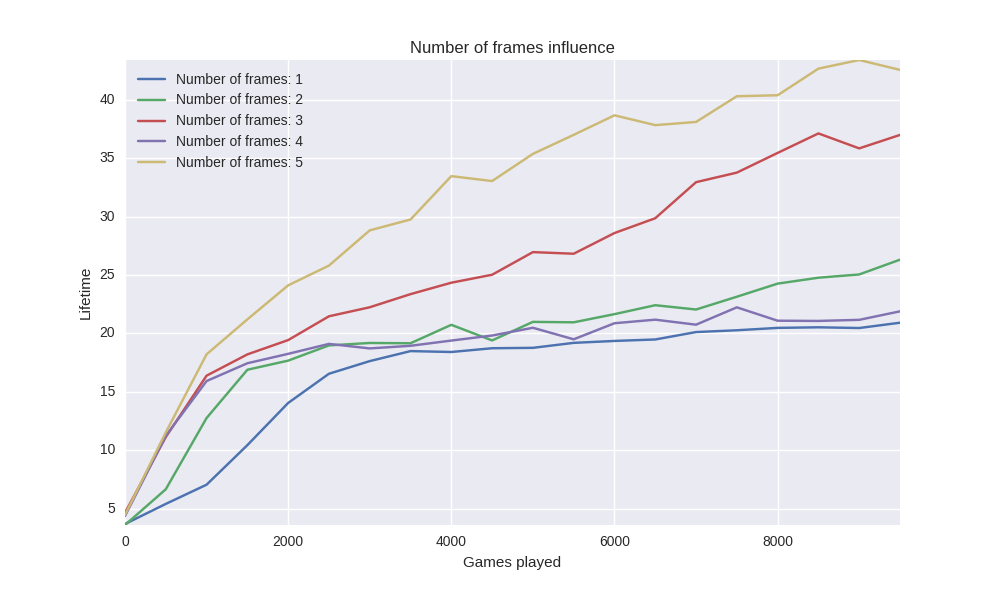
\includegraphics[width=\linewidth]{number_of_frames_dependence.png}
  \caption{Influence of the number of frames fed to the network}
  \label{number_of_frames}
\end{figure}
\end{frame}

\begin{frame}{Results}{Parameter exploration}
\begin{figure}[!htbp]
\centering
  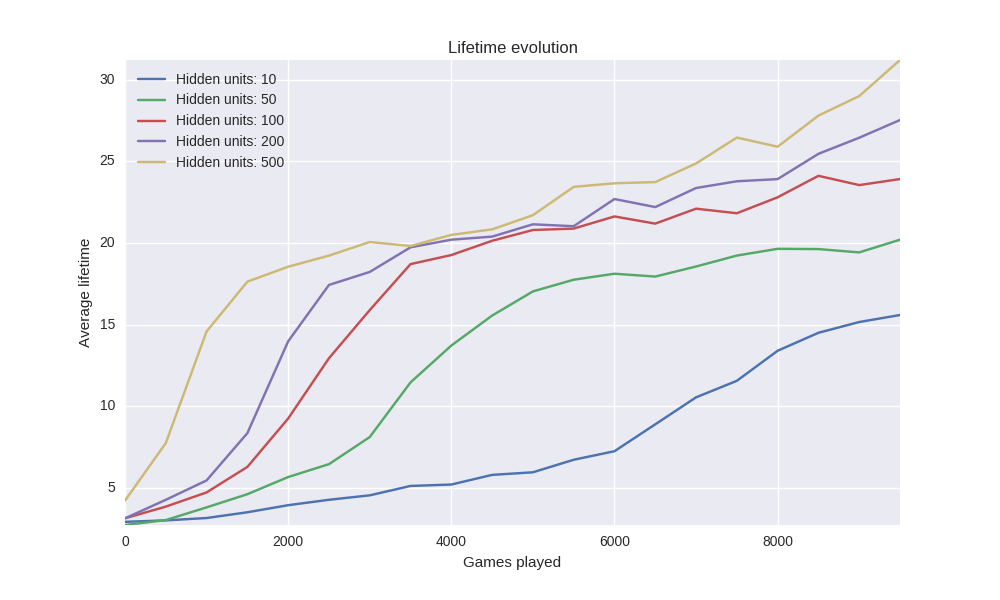
\includegraphics[width=\linewidth]{hidden_units_dependence.png}
  \caption{Influence of the number of hidden units}
  \label{hidden_units}
\end{figure}
\end{frame}



\begin{frame}{Conclusion \& Perspectives}

\begin{itemize}
\item Deep Reinforcement techniques yield promising results to play games which require good reflexes and a bit of a long-time strategy
\item After training over thousands of games, our snake  eats fruits consistently until it grown too much and is eventually stuck by its own body 
\item Real-world applications (e.g. robotics)
\end{itemize}
% Applying deep policy networks to the game of Snake, we have shown that Deep Reinforcement techniques yield promising results to play games which require good reflexes and a bit of a long-time strategy (eating fruits, not being cornered and stuck while the snake keeps growing). 
\end{frame}

\begin{frame}{}
  \begin{center}
  \Huge Thank you for listening !\\Any questions ?
  \end{center}
\end{frame}

\section*{References}
\begin{frame}{References}
% bibliography
\bibliographystyle{unsrt}
\bibliography{bibliography}
\end{frame}

\end{document}

